\documentclass[11pt, oneside]{article}   	% use "amsart" instead of "article" for AMSLaTeX format
\usepackage{geometry}                		% See geometry.pdf to learn the layout options. There are lots.
\geometry{letterpaper}                   		% ... or a4paper or a5paper or ... 
%\geometry{landscape}                		% Activate for for rotated page geometry
%\usepackage[parfill]{parskip}    		% Activate to begin paragraphs with an empty line rather than an indent
\usepackage{graphicx}				% Use pdf, png, jpg, or eps� with pdflatex; use eps in DVI mode
								% TeX will automatically convert eps --> pdf in pdflatex		
\usepackage{amssymb}
\usepackage{amsmath}
\usepackage{parskip}
\usepackage{color}
\usepackage{hyperref}

\title{Integrate z squared}
%\author{The Author}
%\section{}
%\subsection*{}
\date{}							% Activate to display a given date or no date

\graphicspath{{/Users/telliott_admin/Dropbox/Tex/png/}}
% \begin{center} 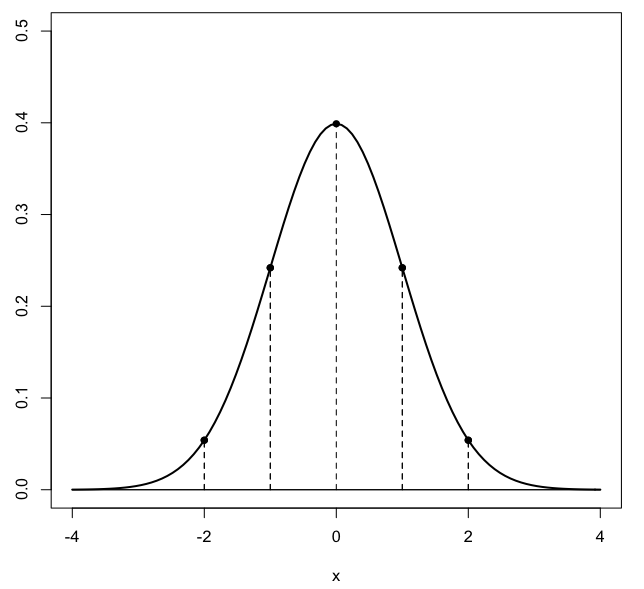
\includegraphics [scale=0.4] {gauss3.png} \end{center}
\begin{document}
\maketitle
\Large

Consider $f(z) = z^2$.  For the path, take the unit circle over the first quadrant from $(1,0)$ to $(0,1)$.  There is an easy way to do this, and a hard way. 

Let's start by checking that this function is analytic, and then doing the hard way first.

Write $z$ in terms of $x$ and $y$:
\[ z = x + iy \]
\[ z^2 = (x + iy)^2 = x^2 - y^2 + i2xy \]
\[ u_x = 2x = v_y \]
\[ u_y = -2y = -v_x \]
The CRE hold.

Also
\[ dz = dx + i \ dy \]
So
\[ \int z^2 \ dz = \int (x^2 - y^2 + 2ixy) ( dx + i \ dy) \]
\[ = \int (x^2 - y^2) \ dx - \int 2 xy \ dy + i \int 2xy \ dx + i \int (x^2-y^2) \ dy \]
As before, we must parametrize this using the relationship between $x$ and $y$ along the curve.
\[ x = \cos t \]
\[ y = \sin t \]
\[ dx = - \sin t \ dt \]
\[ dy = \cos t \ dt \]
and then
\[ x^2 - y^2 = \cos^2 t - \sin^2 t = \cos 2t \]
\[ 2xy = 2 \cos t \sin t = \sin 2t \]
so the integral is
\[ = \int -\cos 2t \  \sin t \ dt - \int \sin 2t \ \cos t \ dt + \dots \]
\[ + \ i \ [ \ \int - \sin 2t \ \sin t \ dt + \int \cos 2t \ \cos t \ dt \]

Looks pretty wild!  In the book they use some trig identities I hadn't seen before, namely starting with the standard
\[ \sin s + t = \sin s \cos t + \sin t \cos s  \]
\[ \cos s + t = \cos s \cos t - \sin s \sin t \]
then, if $s = 2t$ then
\[ \sin 3t = \sin 2t \cos t + \sin t \cos 2t \]
\[ \cos 3t = \cos 2t \cos t - \sin 2t \sin t \]
Looking at the real part of the integral we had (combining terms)
\[ \int -\cos 2t \  \sin t - \sin 2t \ \cos t \ dt = \int - \sin 3t \ dt = \frac{\cos 3t}{3} \]
and for the imaginary part of the integral
\[ i \ [ \ \int - \sin 2t \ \sin t + \cos 2t \ \cos t \ dt = i \int \cos 3t \ dt = i \frac{\sin 3t}{3} \]
That looks a lot better.
\[ \frac{\cos 3t}{3} + i \frac{\sin 3t}{3} \ \bigg |_0^{\pi/2} = - \frac{1}{3} - i \frac{1}{3} = - \frac{1}{3} (1 + i) \]

For one version of the easy way, since $z^2$ is analytic, we can just treat $z$ as if it were a real variable
\[ \int z^2 \ dz = \frac{z^3}{3} \ \bigg |_1^i = - \frac{1}{3} i - \frac{1}{3} \]
Note that if we go all the way around the unit circle the integral is just zero.

Alternatively, parametrize the unit circle as $z = e^{i\theta}$, then $dz = i e^{i\theta} \ d \theta$ and
\[ \int z^2 \ dz = \int e^{i2\theta} \ i \ e^{i\theta} \ d \theta \]
\[ = i \int \ e^{i3\theta} \ d \theta \]
\[ = \frac{1}{3} \ e^{i3\theta} \ \bigg |_{\theta_1}^{\theta_2} \]
From Euler's identity:
\[ e^{i3\theta} = \cos 3 \theta + i \sin 3 \theta \]
If 
\[ \theta_2 = \theta_1 + 2 \pi \]
(going all the way around, the integral is zero).  Over the first quadrant only, we have
\[  e^{i3\theta} \ \bigg |_{0}^{\pi/2} = \cos 3\pi/2 + i \sin 3\pi/2 - \cos 0 - i \sin 0 \]
\[ = 0 + i (-1) - 1 - i(0) = -(1 + i) \]
Multiply by the factor of $1/3$, and we match the previous result.

\end{document}  